% Modern editorial, markup and figure/layout contributions: CC-BY-SA-4.0.
% Historical text and illustrations: Leonhard Euler (1744), public domain.
% Component scope and upstream attribution: see RIGHTS.md.
% Tabula I Fig.4: incidence and labels retained, schematic coordinates.
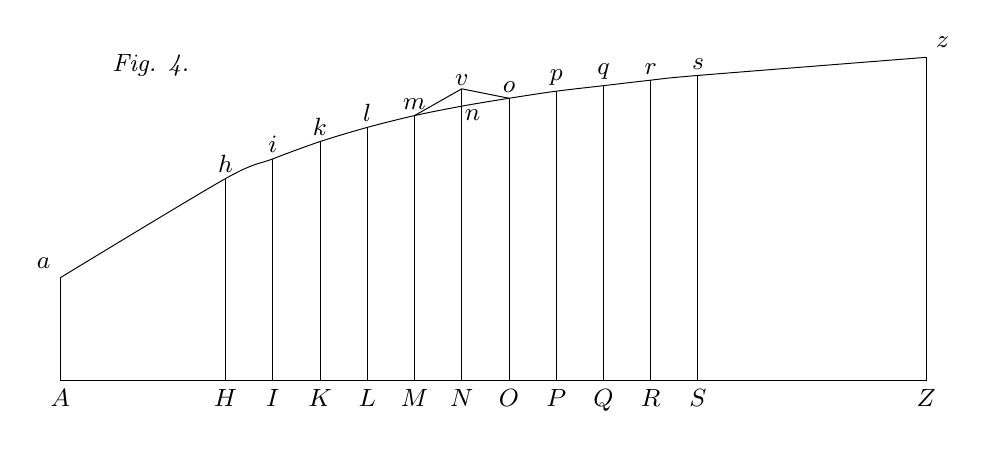
\begin{tikzpicture}[x=1cm,y=1cm,line width=.35pt,font=\small]
\draw (0,0)--(11,0)--(11,4.1);
\draw (0,0)--(0,1.3);
\draw plot[smooth] coordinates {(0,1.3) (2.1,2.56) (2.7,2.81) (3.3,3.03) (3.9,3.21) (4.5,3.36) (5.1,3.48) (5.7,3.58) (6.3,3.67) (6.9,3.74) (7.5,3.81) (8.1,3.87) (11,4.1)};
\node[below] at (0,0) {$A$};\node[above left] at (0,1.3) {$a$};
\node[below] at (11,0) {$Z$};\node[above right] at (11,4.1) {$z$};
\foreach \x/\y/\a/\b in {2.1/2.56/H/h,2.7/2.81/I/i,3.3/3.03/K/k,3.9/3.21/L/l,4.5/3.36/M/m,5.1/3.48/N/n,5.7/3.58/O/o,6.3/3.67/P/p,6.9/3.74/Q/q,7.5/3.81/R/r,8.1/3.87/S/s}{
 \draw (\x,0)--(\x,\y);\node[below] at (\x,0) {$\a$};
 \ifdim\x pt=5.1pt\node[below right,inner sep=1pt] at (\x,\y) {$\b$};\else\node[above,inner sep=2pt] at (\x,\y) {$\b$};\fi
}
\draw (4.5,3.36)--(5.1,3.70)--(5.7,3.58);
\draw (5.1,3.48)--(5.1,3.70);
\node[above,inner sep=1pt] at (5.1,3.70) {$v$};
\node at (1.15,4) {\textit{Fig. 4.}};
\end{tikzpicture}
